% !TeX root = ../dissertation.tex
\appendix

Temporary section for putting graphs that are obsolete or shouldn't be in the final paper,
but which are still useful to look at while writing/editing.

\subsection{Graphics programming model}
In order to support GPUvm and Trillium, we ported and implemented the GPGPU applications
with both CUDA (driver) and OpenCL APIs. Figure~\ref{fig_graphics_api} shows the performance
difference of CUDA and OpenCL (in CUDA toolkit 8.0). It eliminates the concern that OpenCL
has significant performance regression: the execution time of OpenCL kernel and
CUDA kernel are quite close.

OpenCL runtime usually takes much longer time for \texttt{Init} phase mainly because it costs more
to create a context on a device. It is also due to the kernel Just-In-Time compilation in OpenCL.
There is also (fluctuating) small difference in \texttt{Memcpy} time.

\begin{figure}[!th]
	\centering
	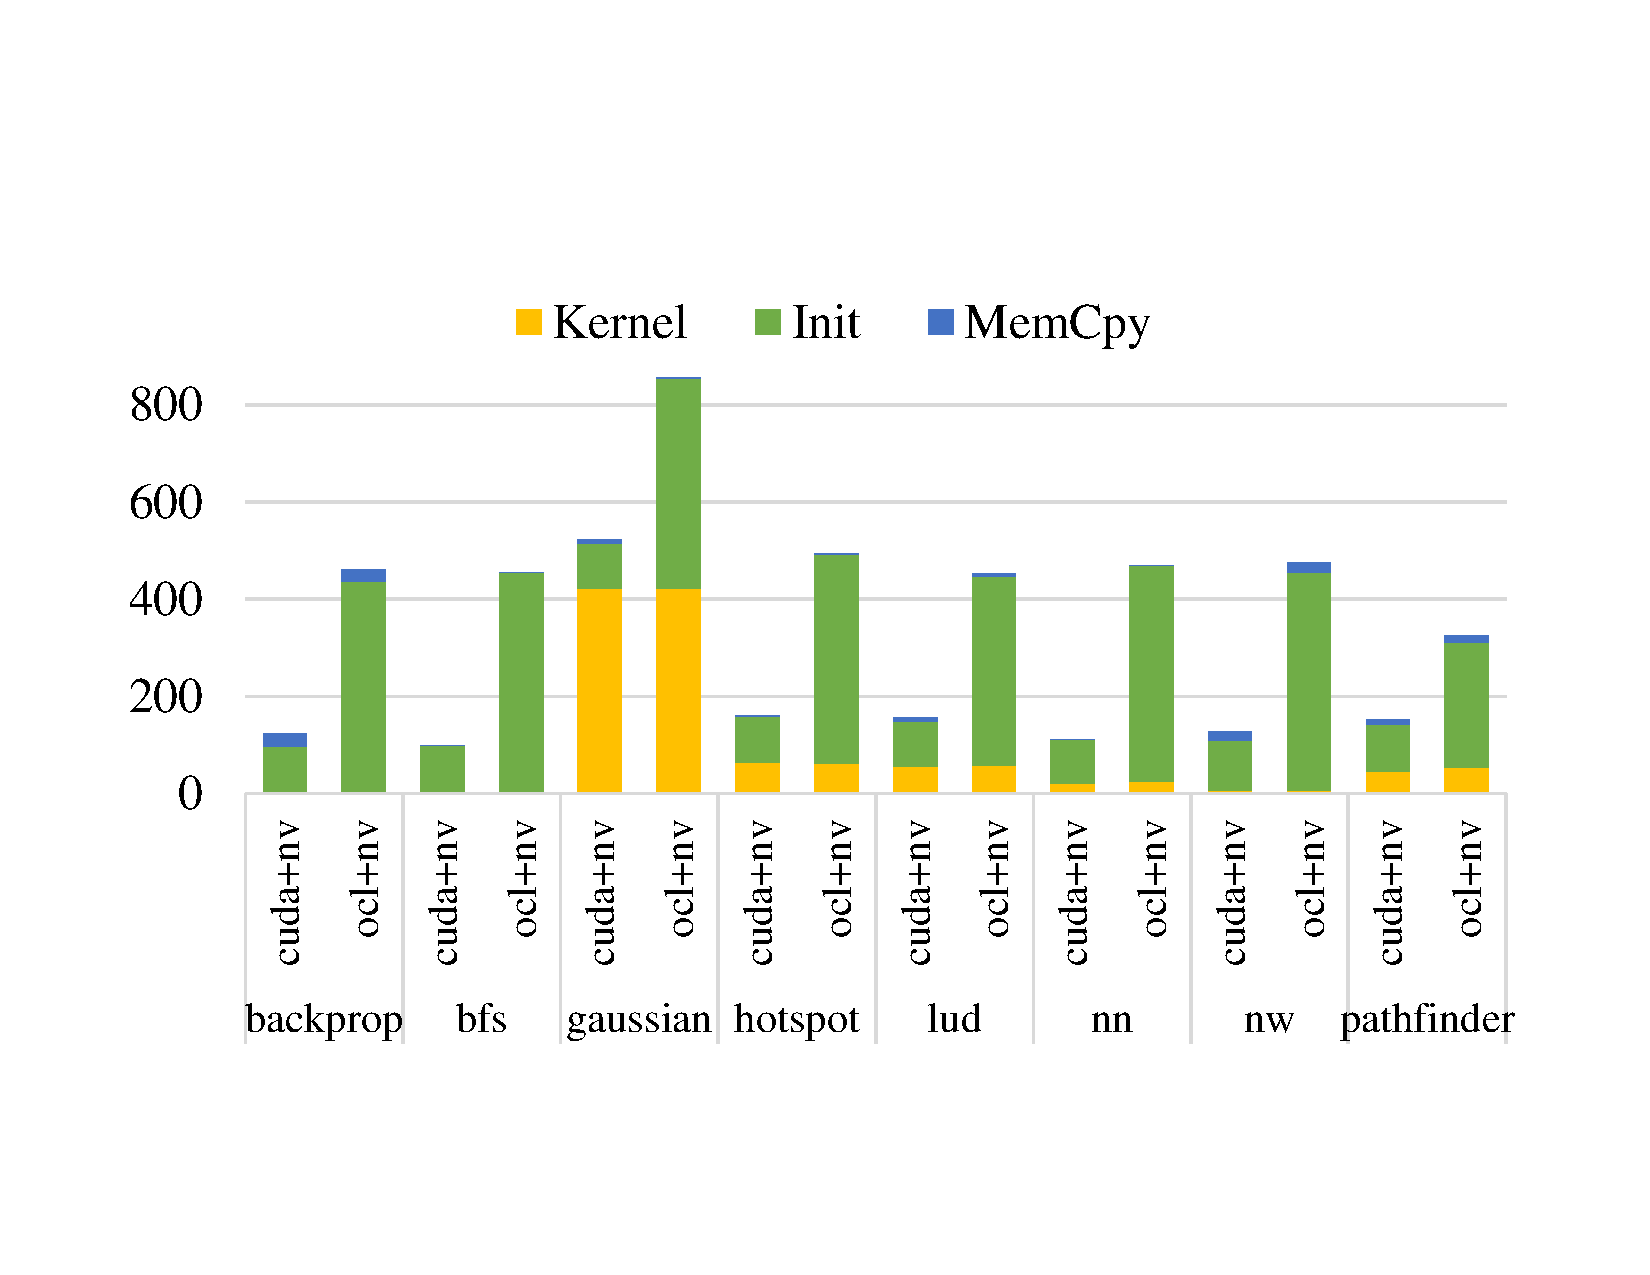
\includegraphics[width=\linewidth,trim={2.2cm 3.8cm 2cm 4cm},clip]{data/basic/graphics_api.pdf}
	\caption{{\footnotesize Runtime of GPGPU applications using CUDA and OpenCL APIs (milliseconds).\cjr{move to methodology, potentially aggregate.}}}
	\label{fig_graphics_api} \end{figure}

	\subsection{Back-end hardware}
GPU virtualization causes some overheads, while some workloads run even faster on CPU than GPU.
Therefore, by utilizing the OpenCL support of Intel CPU, forwarding API calls to run on CPU
may lead to benefits. Figure~\ref{fig_hardware} shows the performance of same benchmarks on
NVIDIA GPU (Quadro 6000) and . The experiment shows that CPU outperforms
GPU on some kind of workloads such as Gaussian Elimination. \texttt{Init} takes longer on GPU,
while copying data is not necessary to be faster from/to CPU\footnote{\textit{Dual copy engines} are
introduced in Fermi architecture.}.

PCIe bus also affects the performance of \texttt{Init} significantly. Our experiment shows
a 6x slowdown using Xen PCIe bus compared with the physical one.

\begin{figure}[!th]
	\centering
	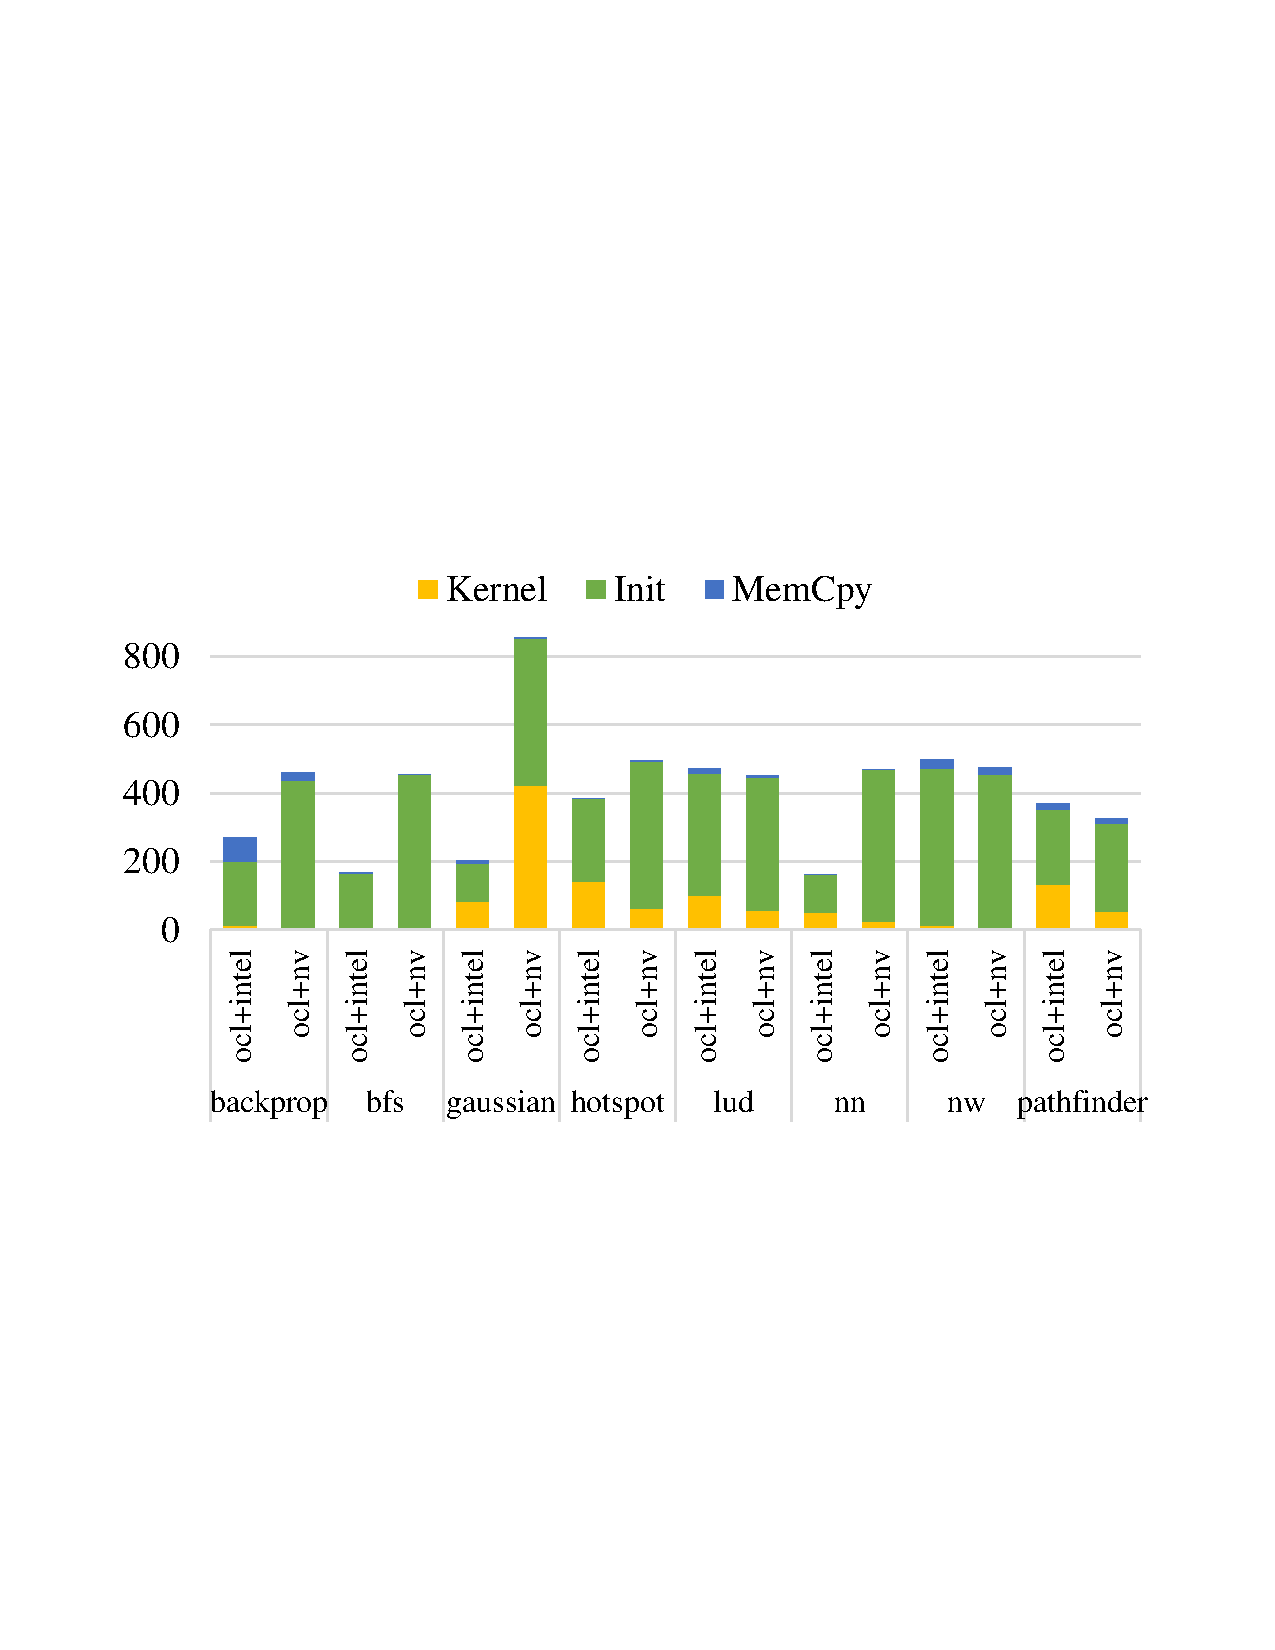
\includegraphics[width=\linewidth,trim={2cm 9cm 2cm 8cm},clip]{data/basic/hardware.pdf}
	\caption{{\footnotesize Runtime of OpenCL applications on Intel CPU and NVIDIA GPU (milliseconds).\cjr{merge into top level graph, relabel with virt design.} \hyu{This one is not in the top level graph. Only CUDA+NV is included there.}}}
	\label{fig_hardware} \end{figure}

\begin{figure}[!ht]
	\centering
	\hspace*{-0.75cm}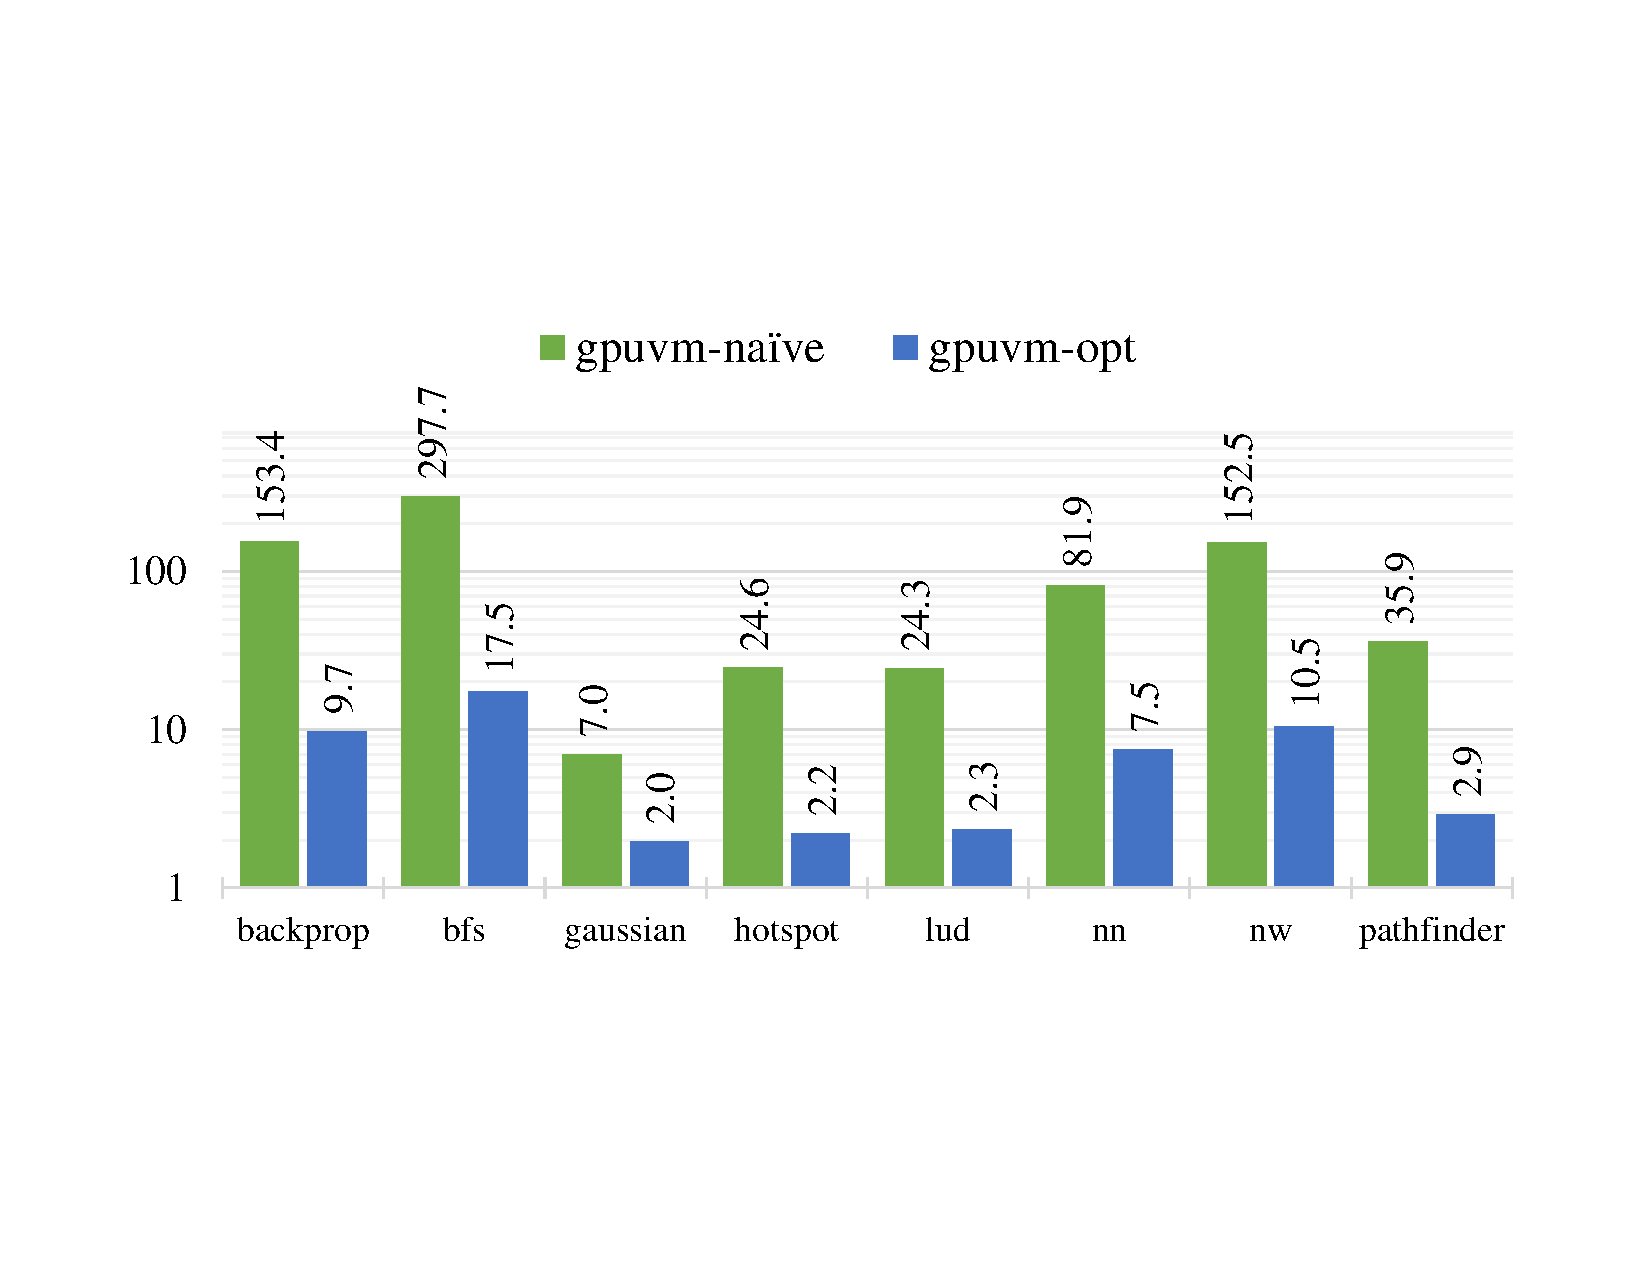
\includegraphics[width=1.1\linewidth,trim={2.2cm 5.5cm 2.2cm 5cm},clip]{data/gpuvm/full-virt_time.pdf}
	\caption{{\footnotesize Relative execution time of the GPU benchmarks on GPUvm. \texttt{CUDA+Gdev} is the baseline.}}
	\label{fig_full-virt_time} \end{figure}

\begin{figure}[!ht]
	\centering
	\hspace*{-0.75cm}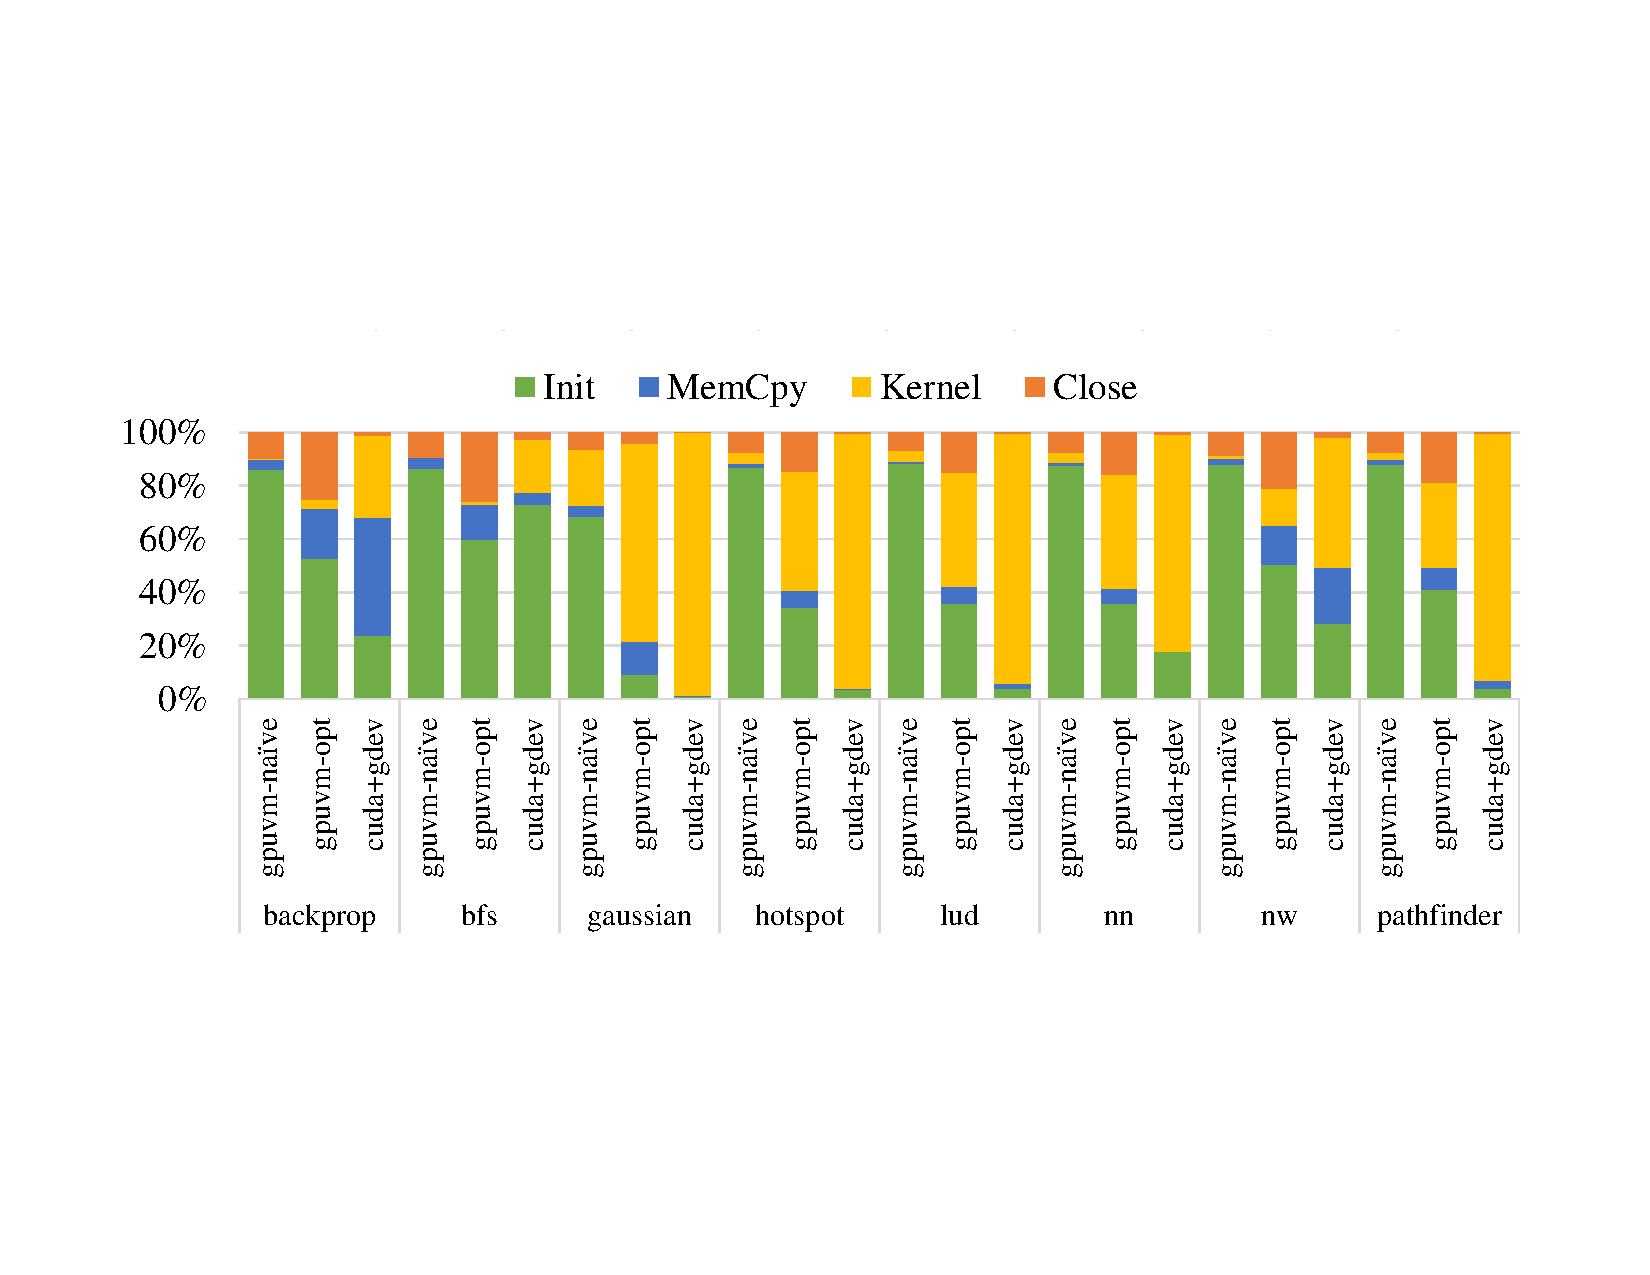
\includegraphics[width=1.1\linewidth,trim={2cm 5.5cm 2.1cm 6.0cm},clip]{data/gpuvm/full-virt_breakdown.pdf}
	\caption{{\footnotesize Runtime breakdown of the GPU benchmarks on GPUvm.}}
	\label{fig_full-virt_breakdown} \end{figure}

\begin{table}[!ht]
	\centering
	\begin{tabular}{l|r|r|r|r|r|}
		\cline{2-6}
		& \multicolumn{1}{l|}{Init} & \multicolumn{1}{l|}{MemCpy} & \multicolumn{1}{l|}{Kernel} & \multicolumn{1}{l|}{Close} & \multicolumn{1}{l|}{Total} \\ \hline
		\multicolumn{1}{|l|}{Na\"ive} & 530x & 125x & 1.03x & 1,020x & 97x \\ \hline
		\multicolumn{1}{|l|}{Opt} & 20x & 50x & 1.03x & 183x & 7x \\ \hline
	\end{tabular}
	\caption{{\footnotesize Overheads of GPUvm in different runtime phases. \texttt{CUDA+Gdev} is the baseline.}}
	\label{tb_gpuvm_overhead}
\end{table}


\begin{figure}[!ht]
	\centering
	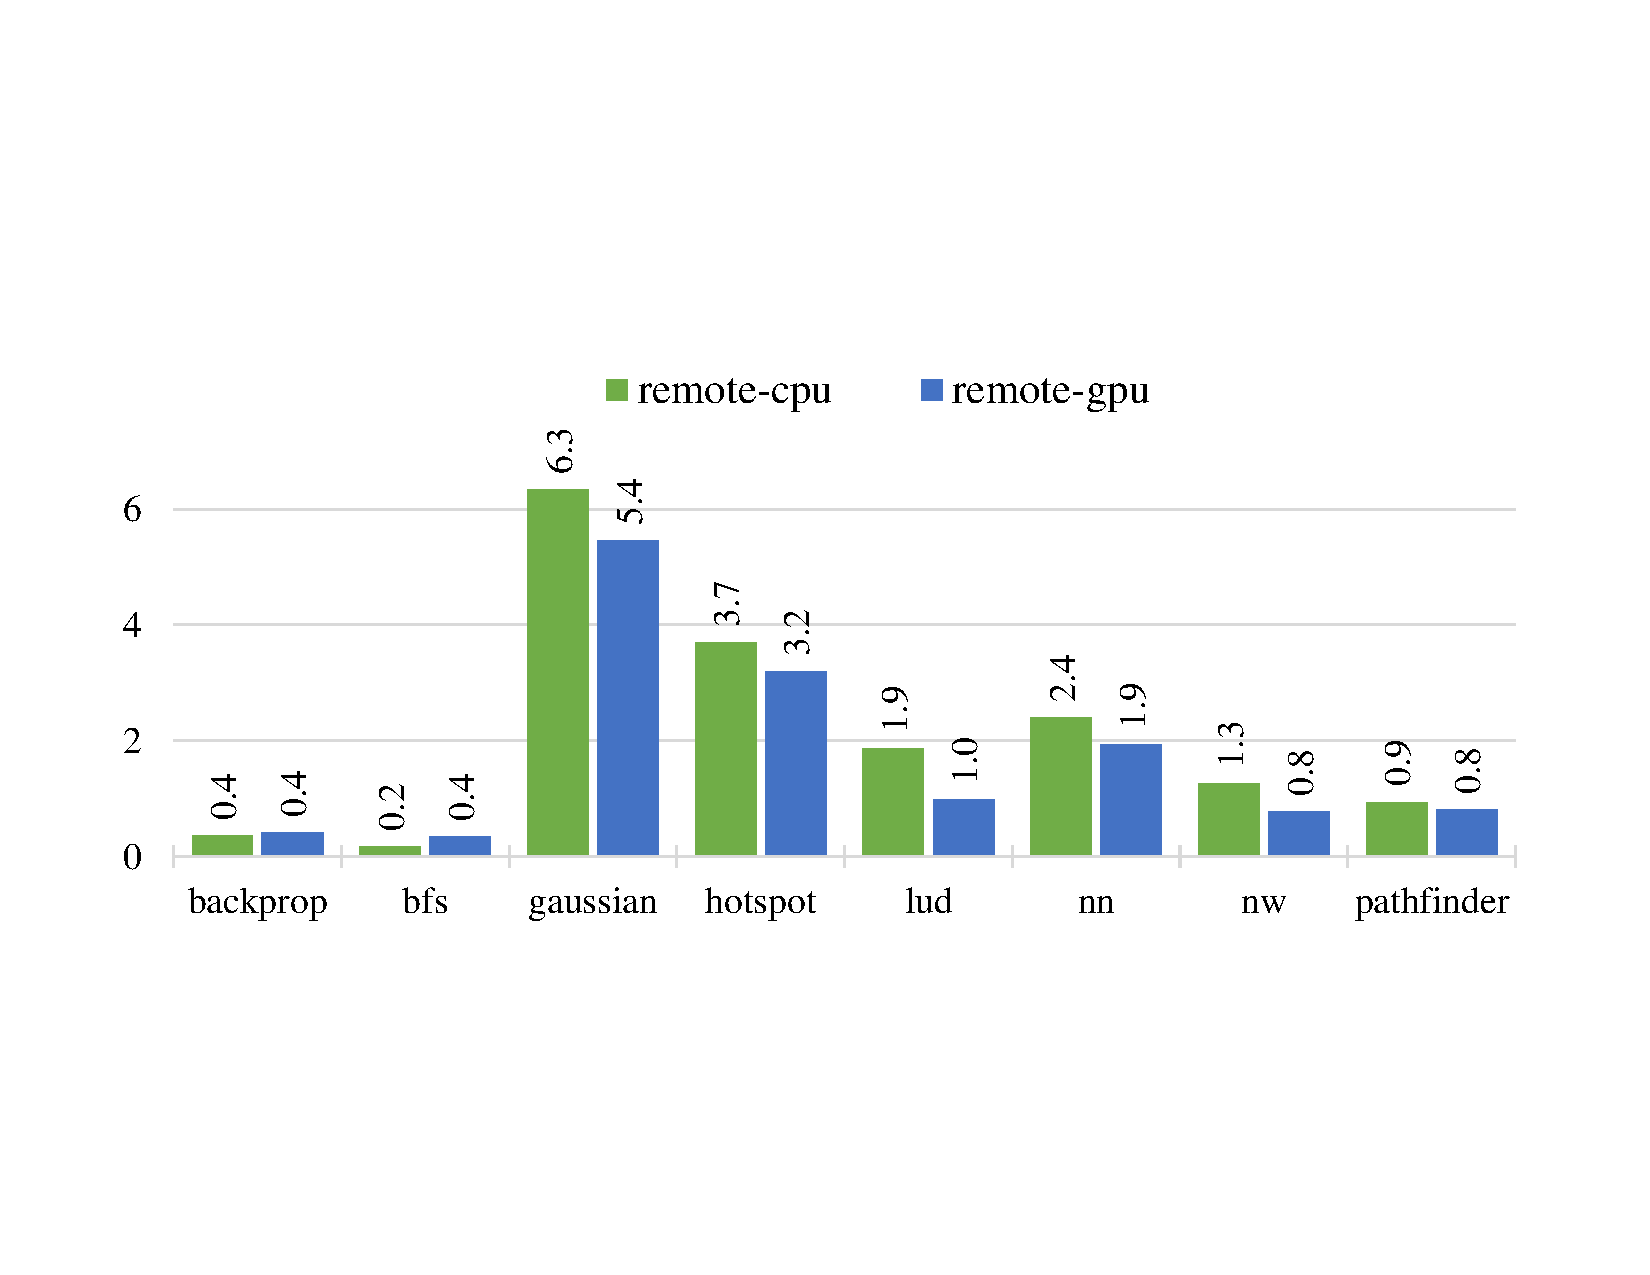
\includegraphics[width=\linewidth,trim={2cm 5.5cm 2.2cm 6cm},clip]{data/api_remote/api_remote_overhead.pdf}
	\caption{{\footnotesize Relative execution time of the OpenCL applications with API remoting to CPU or GPU. \texttt{OCL+NV} is the baseline.}}
	\label{fig_api_remote_overhead} \end{figure}

\begin{figure}[!ht]
	\centering
	\hspace*{-0.25cm}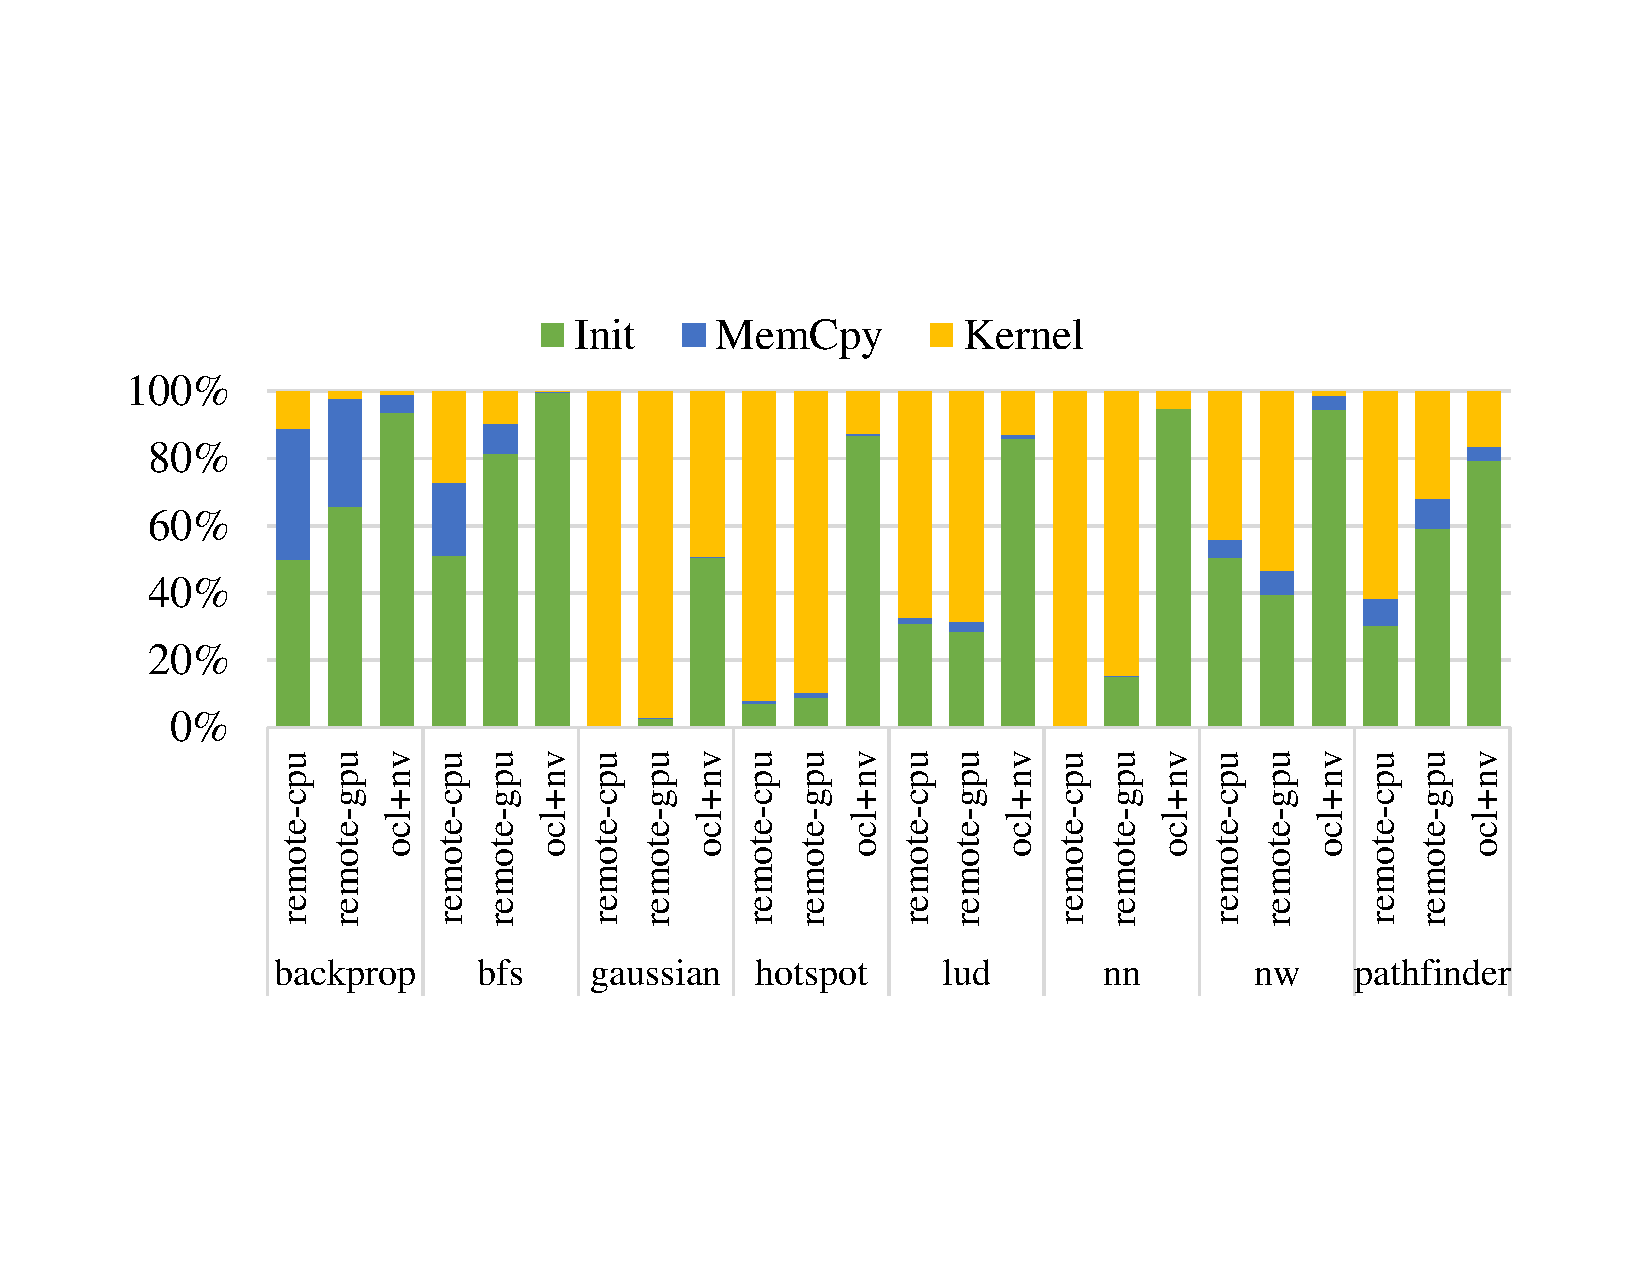
\includegraphics[width=1.1\linewidth,trim={2.2cm 4.8cm 2.1cm 5cm},clip]{data/api_remote/api_remote_breakdown.pdf}
	\caption{{\footnotesize Runtime breakdown of the GPU benchmarks with API remoting.}}
	\label{fig_api_remote_breakdown} \end{figure}

\subsection{Guarantees}

To the extent possible, we'd like to be able to measure any impacts
a design decision has on:

\begin{compactitem}
\item ability to support fairness or QoS,
\item interposition (related to above)
\item compatibility (can the design deal with unmod binaries, etc)
\item isolation (e.g. GPUvm hard-partitions memory, which enables memory protection but not performance isolation.)
\item complexity. Not sure what the right metric is but SLoC is a good start. An ideal set of
	metrics would also somehow measure manageability from an administrator's perspective, and
	programmability (what does support of additional features entail).
\end{compactitem}


\begin{figure}[!ht]
	\centering
	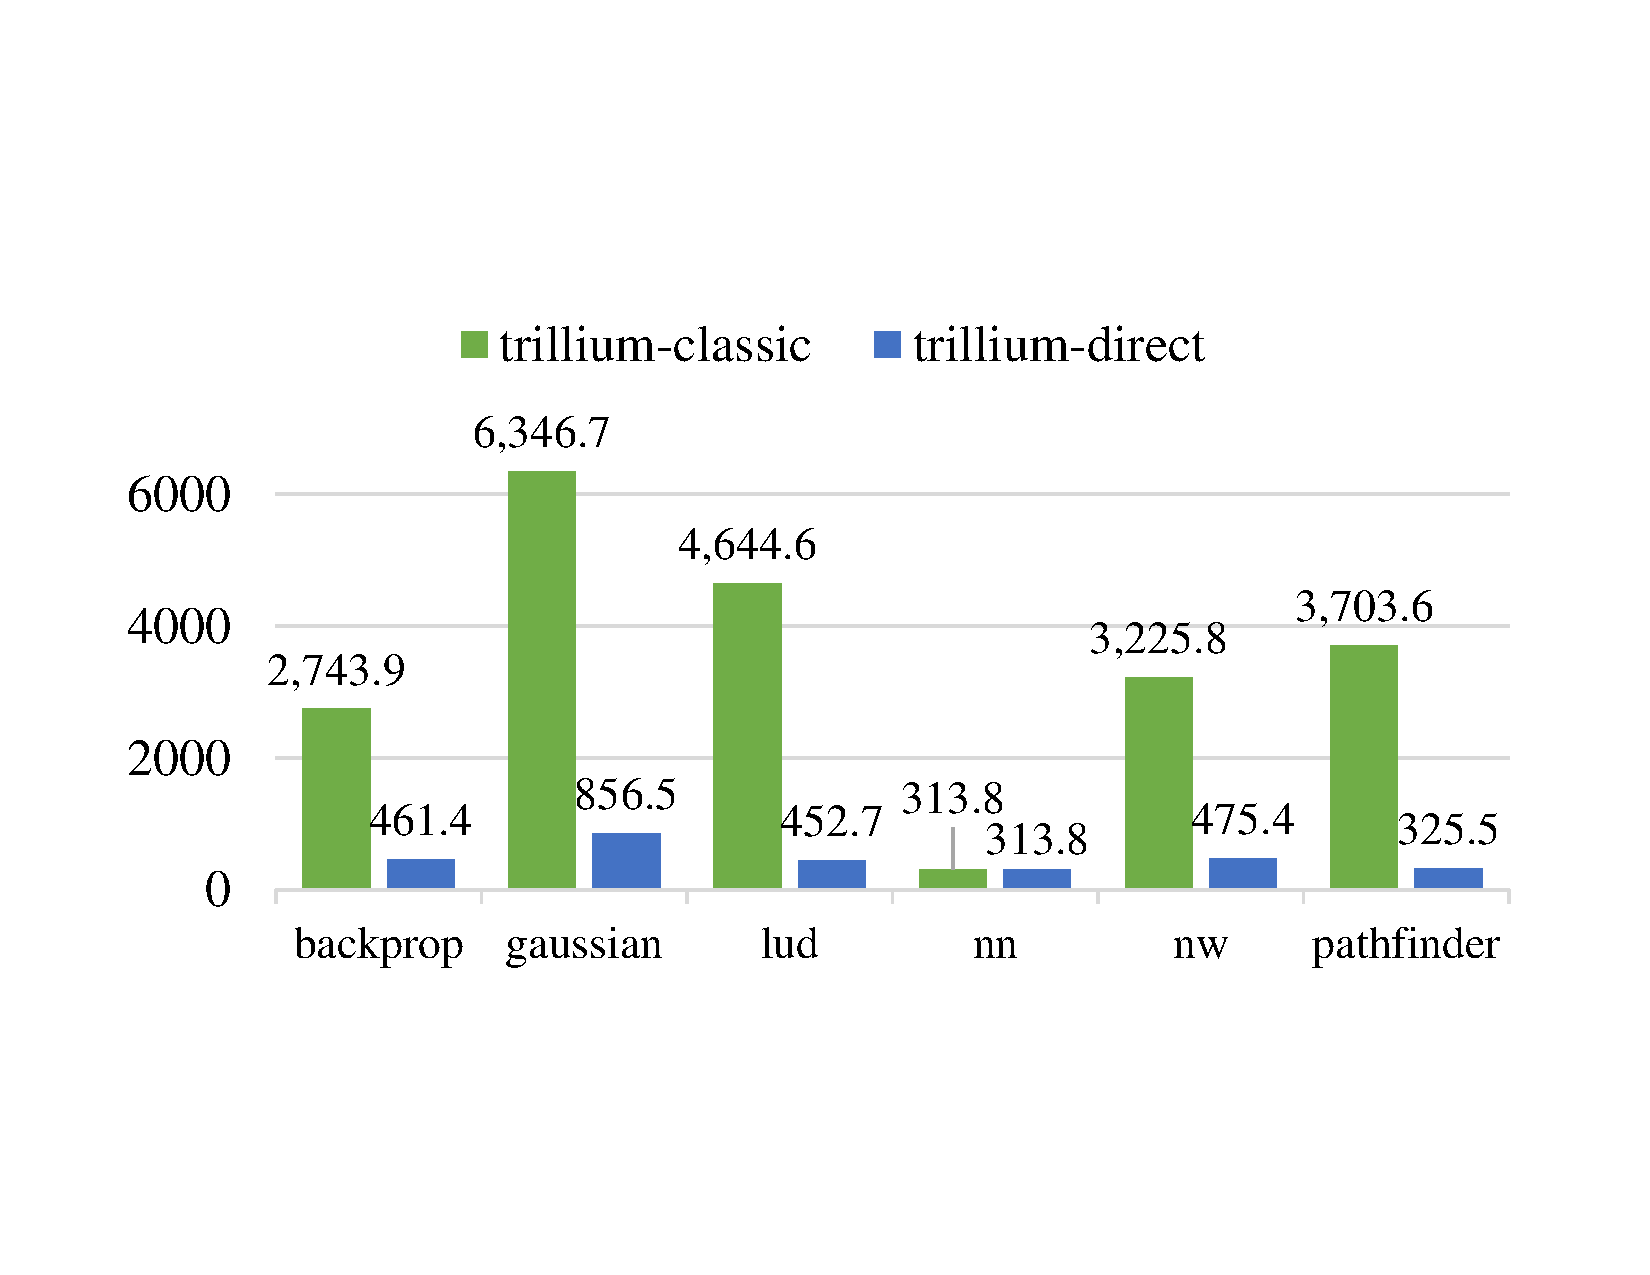
\includegraphics[width=\linewidth,trim={2cm 5cm 2cm 5.5cm},clip]{data/trillium/clover.pdf}
	\caption{{\footnotesize \hyu{Overhead} (seconds). \hyu{Remove me (this figure) please. Check Figure~\ref{fig_trillium_kernel}}}}
	\label{fig_clover_overhead} \end{figure}
